
\documentclass[12pt]{article}
\usepackage[utf8]{inputenc}
\usepackage{amsmath}
\usepackage{graphicx}
\setlength{\parskip}{\baselineskip}%
\setlength{\parindent}{0pt}%

\title{Computational Complexity Assignment 1}

\author{Tyler Tracy}

\begin{document}

\maketitle


\section{Problem 1}


The goal of this turing machine is to use a 3 tape turing machine to detect if a string is a palindrome. The first tape is the input tape, the second tape is used to reverse the input. Then the two tapes are compared against each other to see if they are equal.

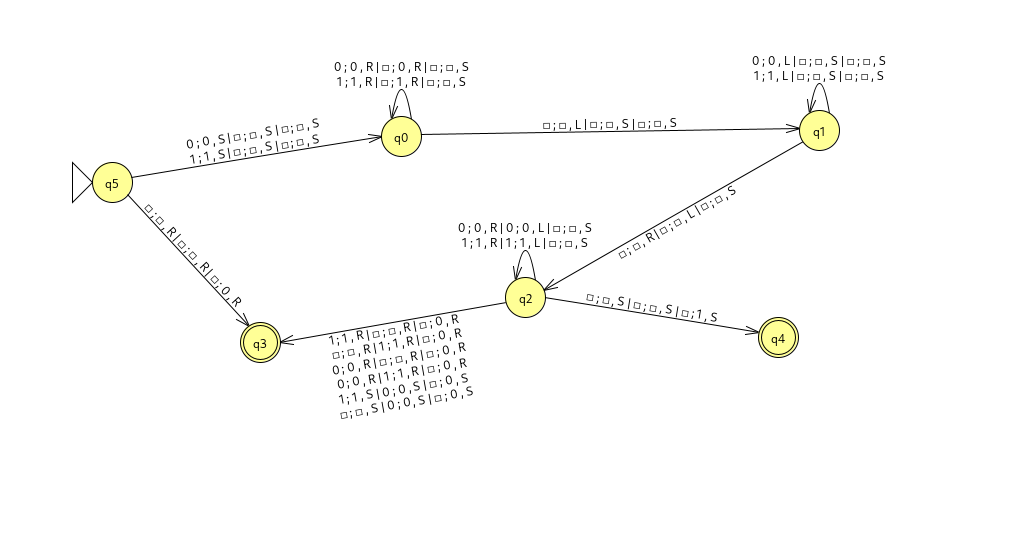
\includegraphics[width=\textwidth]{problem1.png}

The initial check to see if the string is empty is a single operation
The process of reversing the string is $O(n)$ time
The process of comparing the two strings is $O(n)$ time
The total time complexity is $O(n)$

\section{Problem 2}






\end{document}